\documentclass[letterpaper]{article}

% --- Required Packages ---
\usepackage{parskip}            % Removes paragraph indentation, adds space between paragraphs
\usepackage[unicode, draft=false]{hyperref} % Setup hyperref package, and colours for links
\usepackage{titlesec}           % For custom section formatting
\usepackage{fancyhdr}           % Required for custom headers and footers
\usepackage{extramarks}         % Required for \lastxmark in the footer
\usepackage{enumitem}           % For nice lists (bullet points)
\usepackage[backend=biber, style=numeric]{biblatex}
\addbibresource{references.bib}
\RequirePackage{graphicx}
% --- Lab Details Variables ---
\newcommand{\labTitle}{ML in Security and Privacy}
\newcommand{\labDueDate}{April 17th, 2026}
\newcommand{\labClass}{CSC429}
\newcommand{\labClassTime}{}
\newcommand{\labClassInstructor}{Professor Fang}
\newcommand{\labAuthorName}{\textbf{Helen Huy, McCay Rudick, Jess Alencaster}}

% --- Basic Document Settings ---
\topmargin=-0.45in
\evensidemargin=0in
\oddsidemargin=0in
\textwidth=6.5in
\textheight=9.0in
\headsep=0.25in

\linespread{1.1}

% --- Header and Footer Settings ---
\pagestyle{fancy}
\lhead{\labAuthorName}
\rhead{\labClass\ (\labClassInstructor\ \labClassTime): \labTitle}
\lfoot{\lastxmark}
\cfoot{\thepage}

\renewcommand\headrulewidth{0.4pt}
\renewcommand\footrulewidth{0.4pt}

\setlength\parindent{0pt}

% --- Custom Section Formatting  ---
\titleformat{\section}{\Large\bfseries\raggedright}{}{0em}{}[\titlerule]
\titlespacing{\section}{0pt}{10pt}{5pt}
\titleformat{\subsection}{\large\bfseries\raggedright}{}{0em}{}
\titlespacing{\subsection}{0pt}{8pt}{3pt}

\begin{document}
\thispagestyle{empty}

% --- Title Block ---

\vspace*{\fill}
\begin{center}
    {\Huge \scshape \labClass: \labTitle} \\ \vspace{10pt}
    {\Large \labAuthorName} \\ \vspace{5pt}
    {\large \labClassInstructor \ \labClassTime} \\ \vspace{5pt}
    {\large Due Date: \labDueDate}
\end{center} 
\vspace*{\fill}

\newpage
% BEGIN LAB CONTENT

\section{1. Open-Source Data Resources}

\subsection*{Resource 1: Kaggle} 
\textbf{Link:} \href{https://www.kaggle.com/}{Kaggle Platform} \\
Kaggle is a collaborative machine learning platform that hosts a vast repository of public datasets, competitions, and user-published code for various projects.
\begin{itemize}
    \item \textbf{Advantages/Disadvantages:} A major advantage is the massive variety of available datasets, complete with community discussion boards, shared code notebooks, and dataset "usability" scores to help gauge quality. A disadvantage is that the crowdsourced nature can lead to duplicate or modified versions of original datasets, requiring users to be cautious about data provenance and authenticity.
    \item \textbf{Synthetic or Real Data:} It predominantly hosts real-world data across numerous domains, such as the MNIST database of handwritten digits collected from real Census Bureau employees and high-school students \parencite{mnist}.
    \item \textbf{Main Uses:} It is mostly used for general-purpose ML tasks, rapid prototyping, and evaluating baseline machine learning models on standard datasets.
\end{itemize}

\subsection*{Resource 2: Canadian Institute for Cybersecurity (CIC) Datasets}
\textbf{Link:} \href{https://www.unb.ca/cic/datasets/index.html}{UNB CIC Datasets} \\
The CIC is an academic data repository maintained by the University of New Brunswick (UNB) that provides dynamically generated benchmark datasets specifically designed for network security.
\begin{itemize}
    \item \textbf{Advantages/Disadvantages:} The primary advantage is that it provides highly realistic, complete network captures (in PCAP and CSV formats) with up-to-date, labeled intrusion scenarios, successfully avoiding the heavy anonymization that often limits the utility of other datasets. A disadvantage is that the datasets consist of massive raw network traces (ranging from 4 GB to over 23 GB per day of capture) which can require significant computational overhead and storage to process.
    \item \textbf{Synthetic or Real Data:} It consists of real data generated within a controlled testbed environment. The creators use profiling agents to simulate real human behaviors for naturalistic benign background traffic and execute real-world multi-stage attack scenarios to generate the malicious traffic.
    \item \textbf{Main Uses:} It is mostly used by researchers for training, evaluating, and benchmarking anomaly-based Intrusion Detection Systems (IDS) and other network security applications.
\end{itemize}

\pagebreak
\section{2. Open-Source ML Algorithms}

\subsection*{Classification: Convolutional Neural Network (CNN)}
\textbf{Link:} \href{https://www.tensorflow.org/guide/keras/sequential_model}{Keras Sequential Model} \\
\textbf{Description:} A Convolutional Neural Network (CNN) is a deep learning algorithm that takes input features and passes them through convolutional and pooling operations to detect patterns. 

\textbf{Advantages:} CNNs are highly effective for group-based tasks and extracting spatial hierarchies, making them excellent for image classification tasks. By applying 2D filters, they easily detect edges, textures, and shapes within spatial structures.

\textbf{Disadvantages and Costs:} Generally, CNNs do not perform well on standard network traffic. They are fundamentally designed for grid-based data (like pixels in an image). When attempting to adapt them to tabular or sequential data (like a 1D CNN for network flows), standard pooling operations do not work well or translate effectively for 1D feature arrays. Additionally, training requires significant computational processing power and memory, creating high costs that can be a bottleneck for localized training on small edge devices.

\textbf{Uses and Selection Rationale:} You would choose a CNN to construct a hypothesis around image-based classification (such as evaluating the MNIST or CIFAR-10 datasets \parencite{mnist, cifar10}) because its group-based spatial feature extraction is perfectly suited for visual patterns. Conversely, you would not choose it for raw network traffic analysis where its rigid grid-based assumptions and pooling operations fail to capture the correct features.

\vspace{1em}

\subsection*{Regression: Linear Regression}
\textbf{Link:} \href{https://scikit-learn.org/stable/modules/generated/sklearn.linear_model.LinearRegression.html}{Scikit-Learn Linear Regression} \\
\textbf{Description:} Linear regression is a foundational ML algorithm used to model outcomes based on one or more independent variables by fitting a linear equation to observed data. 

\textbf{Advantages:} It is mathematically simple, highly interpretable, and easily deployed in distributed environments. 

\textbf{Disadvantages and Costs:} It strictly assumes a linear relationship between features and the target variable, meaning it cannot capture complex, non-linear data patterns. It is also highly sensitive to outliers. However, because it is mathematically simple, its computational costs are extremely inexpensive.

\textbf{Uses and Selection Rationale:} You would choose Linear Regression to construct a hypothesis in resource-constrained environments that require predicting a continuous outcome based on strictly linear features. For example, it is used in an Internet of Vehicles (IoV) scenario \parencite{zhao2020} because vehicles must quickly train a local model on simple sensor data, and Linear Regression allows them to do so without exhausting their limited computational resources.

\vspace{1em}

\pagebreak

\subsection*{Clustering: K-Means Clustering}
\textbf{Link:} \href{https://scikit-learn.org/stable/modules/generated/sklearn.cluster.KMeans.html}{Scikit-Learn K-Means} \\
\textbf{Description:} K-Means is an unsupervised ML algorithm that partitions unlabelled data into $K$ distinct clusters based on feature similarity and distance to a centroid \parencite{macqueen1967}.

\textbf{Advantages:} It is fast, easy to implement, and scales exceptionally well to large, unlabelled datasets.

\textbf{Disadvantages and Costs:} The algorithm requires the user to manually pre-define the number of clusters ($K$) before training. It also struggles with non-circular cluster shapes, and its centroids can be heavily skewed by noisy data and outliers. It carries a low to moderate computational cost, which is largely dependent on the size of the dataset and the number of clusters chosen.

\textbf{Uses and Selection Rationale:} You would choose K-Means to construct a hypothesis when the goal is to discover natural groupings within unlabelled data without predicting a specific target. It is chosen for uses like grouping cellular users in a 5G network based on their geographic location and content preferences because it is specifically designed to partition data efficiently based on feature similarity for proactive caching \parencite{liu2020}.

\begin{figure}[h!]
    \centering
    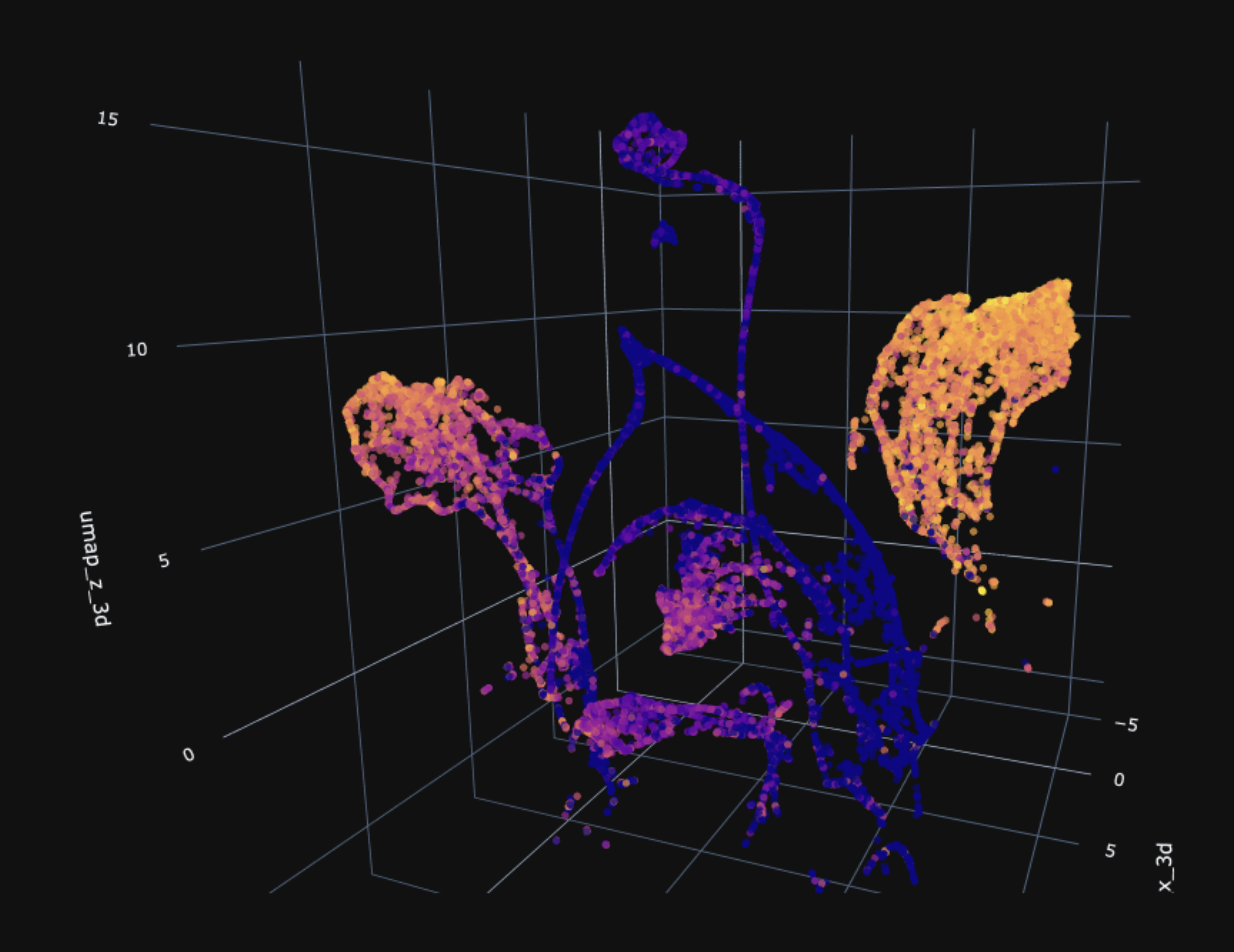
\includegraphics[width=0.4\textwidth]{k-means.png}
    \caption{K Means Clustering Example 3d representation}
\end{figure}

\pagebreak

\section{3. Security and Privacy Applications}

\subsection*{Application 1: Federated learning in IoT devices.}
This application demonstrates how federated learning is used across decentralized IoT networks to collaboratively build machine learning models without centralizing sensitive raw data.

\textbf{Why they used it:} To collaboratively train models on sensitive client data, such as vehicle sensor data or a cellular user's location and content preferences, without exposing the raw data to a central server.

\textbf{How they did it:} Because FL alone cannot introduce a strict mathematical privacy guarantee, researchers integrate noise or encryption. One approach applies a Linear Regression algorithm in an Internet of Vehicles (IoV) environment, where each vehicle trains a model locally and perturbs the gradients with Local Differential Privacy (LDP) noise before uploading them \parencite{zhao2020}. Another method proposes a privacy-preserving federated K-Means clustering scheme \parencite{liu2020}. This uses K-Means to cluster 5G cellular users based on location and preferences, masking the uploaded gradients using secret sharing so the server only updates cluster centroids.

\textbf{How they evaluated it:} The clustering algorithm was evaluated based on its utility in a proactive caching scenario. Evaluations measured the network's ability to successfully pre-download desired content to nearby 5G base stations based on the cluster's taste, validating that performance was maintained without the server ever seeing individual user data.

\subsection*{Application 2: Privacy-preserving intrusion detection in IoT.}
This application focuses on deploying localized machine learning models to detect malicious network traffic in industrial environments while utilizing differential privacy to protect proprietary operational data.

\textbf{Why they used it:} To monitor and classify malicious industrial IoT network traffic (like DoS attacks) locally without transferring proprietary operational data to a central server, which risks exposure.

\textbf{How they did it:} One solution deploys a 1D Convolutional Neural Network (CNN) with an eight-layer architecture to classify IoT traffic locally \parencite{torre2025}. To protect the model updates from membership inference attacks, Laplace-distributed noise is calibrated and added directly to the CNN weights (applying DP) before sharing them with the aggregator. Alternatively, a multinomial logistic regression (softmax regression) algorithm can be used to classify traffic, applying both Laplacian and Gaussian noise mechanisms directly to the model weights to ensure the updates the server receives are differentially indistinguishable \parencite{ruzafa2023}.

\textbf{How they evaluated it:} The 1D CNN was evaluated across seven real-world IoT datasets. Because network intrusion data is often highly imbalanced and overall accuracy is an insufficient metric on its own, the model was evaluated using multi-class, threshold-independent metrics \parencite{torre2025}. Privacy protection was successfully maintained without significantly degrading detection utility, achieving an accuracy of 97.31\%, precision of 95.59\%, recall of 92.43\%, and an F1-score of 92.69\%.

\pagebreak

\subsection*{Application 3: Privacy-preserving federated learning in healthcare.}
This application evaluates the efficacy and vulnerabilities of current federated learning and differential privacy frameworks in protecting highly sensitive patient records within strictly regulated clinical settings.

\textbf{Why they used it:} To ensure patient data privacy in clinical settings to comply with strict regulations like HIPAA and GDPR, where the cost of a poor privacy-utility tradeoff is measured in negative patient outcomes rather than just model performance.

\textbf{How they did it:} Existing DP and FL models used in clinical settings were investigated to determine if the noise calibrated into these models was actually sufficient to protect highly sensitive healthcare data \parencite{teo2024}.

\textbf{How they evaluated it:} The privacy guarantees of these models were evaluated by actively subjecting them to membership inference attacks and reconstruction attacks. Through these evaluations, it was found that adversaries could still successfully infer whether a specific patient’s data was used in the training set, or even reconstruct the original patient record entirely \parencite{teo2024}. This evaluation proved that DP and FL in healthcare is one of the hardest contexts to secure, as standard DP applications remain highly susceptible to leakage.

% \nocite{*}
% --- References ---
\newpage
\section{}

\printbibliography[title={References}]

\end{document}